\documentclass[english]{lni}

\IfFileExists{latin1.sty}{\usepackage{latin1}}{\usepackage{isolatin1}}

\usepackage{graphicx}

\newcommand{\ignore}[1]{}

\begin{document}

\author{S\'ergio A. de Carvalho Jr.\,$^{\rm a,b,c}$ and Sven Rahmann\,$^{\rm b,c}$}
\title{Microarray Layout as a Quadratic Assignment Problem}

%% no address command?
%% \address{$^{\rm a}$Graduiertenkolleg Bioinformatik, Bielefeld University, Germany,\\
%% $^{\rm b}$International NRW Graduate School in Bioinformatics and Genome Research,
%% Bielefeld University, Germany,\\
%% $^{\rm c}$Algorithms and Statistics for Systems Biology group, Genome Informatics,
%% Technische Fakult\"at, Bielefeld University, D-33594 Bielefeld, Germany.}

\maketitle

% ==============================================================================
\begin{abstract}
% ==============================================================================

The production of commercial DNA microarrays is based on a
light-directed chemical synthesis driven by a set of masks or
micromirror arrays. Because of the natural properties of light and the
ever shrinking feature sizes, the arrangement of the probes on the
chip and the order in which their nucleotides are synthesized play an
important role on the quality of the final product.
We propose a new model called \emph{conflict index} for evaluating
microarray layouts, and we show that the probe placement problem is an
instance of the \emph{quadratic assignment problem} (QAP), which opens
up the way for using QAP heuristics. We use a existing heuristic
called GRASP to design the layout of small artificial chips with
promising results. We compare this approach with the best known
algorithm and describe how it can be combined with other existing
algorithms to design the latest million-probe microarrays.

\end{abstract}

% ==============================================================================
\section{Introduction}
% ==============================================================================

An oligonucleotide microarray is a piece of glass or plastic on which
single-stranded fragments of DNA, called \emph{probes}, are affixed or
synthesized. The chips produced by Affymetrix, for instance, can contain more
than one million spots (or \emph{features}) as small as 11 $\mu$m, with each
spot accommodating several million copies of a probe. Probes are typically 25
nucleotides long and are synthesized in parallel, on the chip, in a series of
repetitive steps. Each step appends the same nucleotide to probes of selected
regions of the chip. Selection occurs by exposure to light with the help of a
photolithographic mask that allows or obstructs the passage of light
accordingly \cite{FODOR91}.

Formally, we have a set of probes $\mathcal{P} = \{p_{1}, p_{2}, ... p_{n}\}$
that are produced by a series of masks
$\mathcal{M} = (m_{1}, m_{2}, ... m_{\mu})$, where each mask $m_{k}$ induces the
addition of a particular nucleotide $t_{k} \in \{A, C, G, T\}$ to a subset
of~$\mathcal{P}$. The \emph{nucleotide deposition sequence}
$\mathcal{S} = t_{1} t_{2} \ldots t_{\mu}$ corresponding to the sequence of
nucleotides added at each masking step is therefore a supersequence of all
$p_{i} \in \mathcal{P}$ \cite{RAHMANN03}.

In general, a probe can be \emph{embedded} within $\mathcal{S}$ in several ways.
An embedding of $p_{i}$ is a $\mu$-tuple
$\varepsilon_{i} = (e_{i,1}, e_{i,2}, ... e_{i,\mu})$ in which $e_{i,k} = 1$ if
probe $p_{i}$ receives nucleotide $t_{k}$ (at step~$k$), or 0 otherwise
(Figure~\ref{fig:masking_process}).
The deposition sequence is often taken as a repeated permutation of the
alphabet, mainly because of its regular structure and because such sequences
maximize the number of distinct subsequences. \ignore{ \cite{CHASE76}.}

\begin{figure}
\centerline{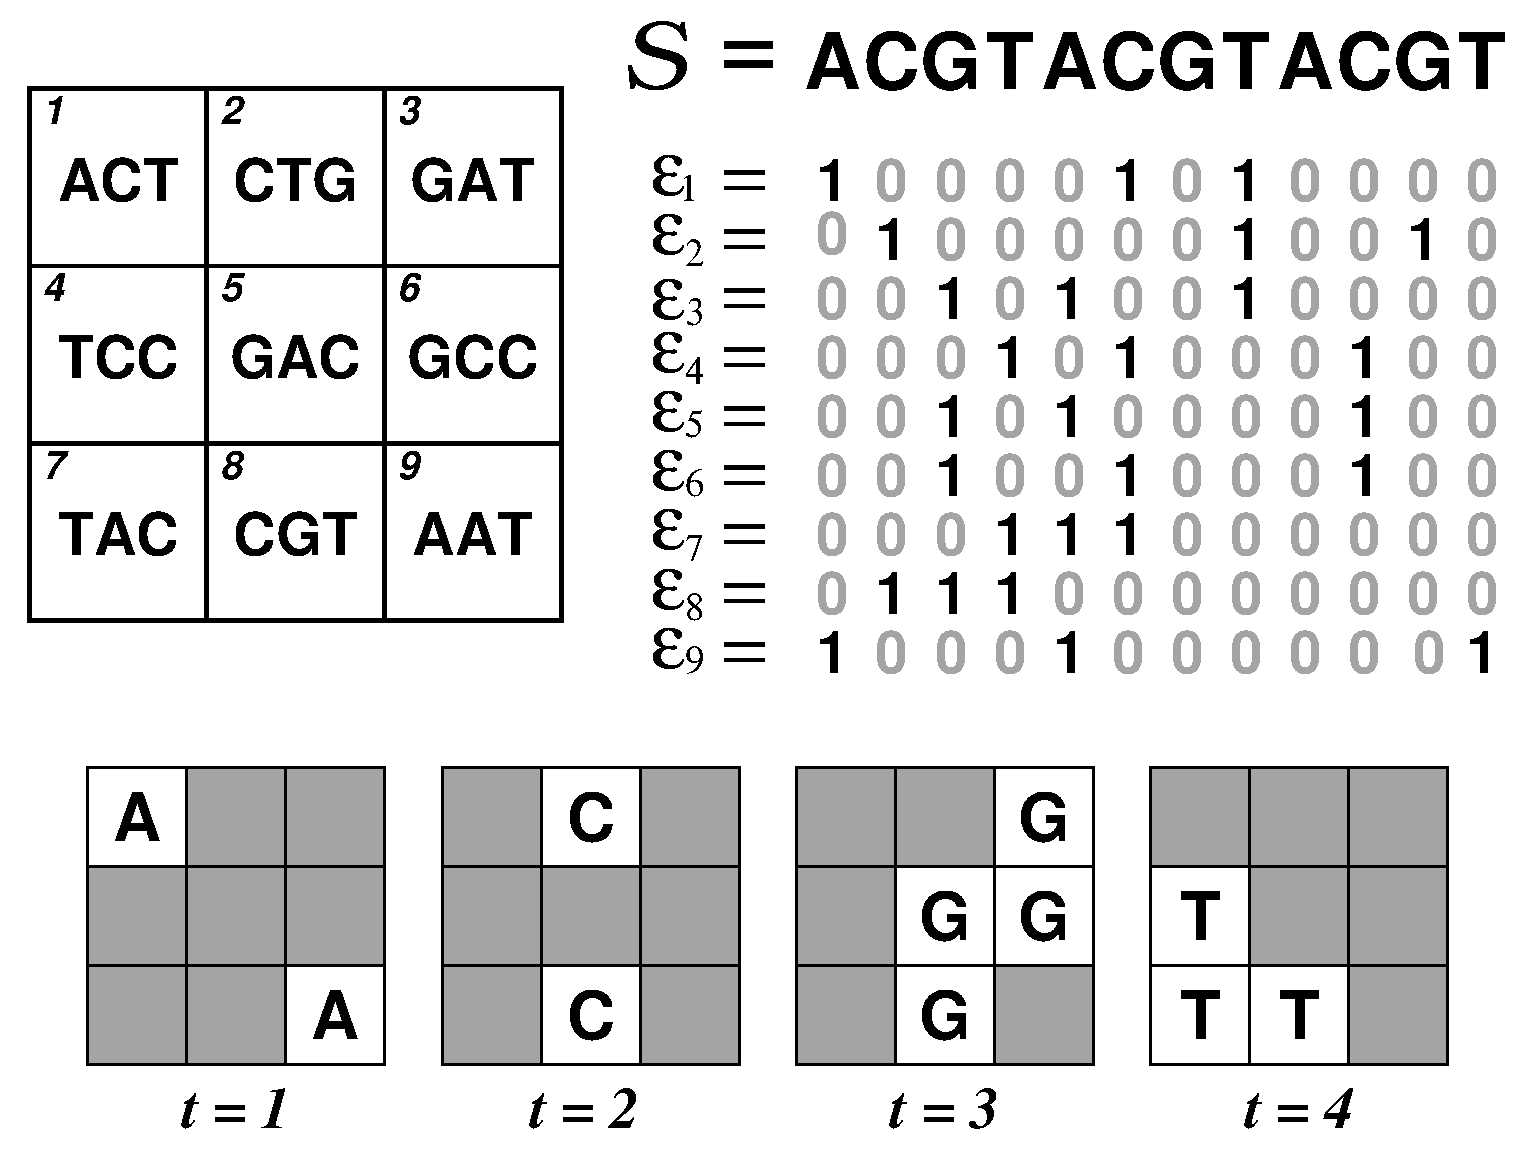
\includegraphics[width=230pt]{chip}}
\caption{Synthesis of a hypothetical 3$\times$3 chip. Top left: chip
layout and the 3~nt probe sequences. Top right: deposition
sequence and probe embeddings. Bottom: first four resulting masks.}
\label{fig:masking_process}
\end{figure}

We distinguish between \emph{synchronous} and \emph{asynchronous} embeddings.
In the first case, each probe has exactly one nucleotide synthesized in every
cycle of the deposition sequence; hence, 25 cycles or 100 steps are needed to
synthesize probes of length 25. In the case of asynchronous embeddings,
probes can have any number of nucleotides synthesized in any given cycle,
allowing shorter deposition sequences. All Affymetrix chips that we know of
can be asynchronously synthesized in 74 steps (18.5 cycles), which is probably
due to careful probe selection.

Because of diffraction of light or internal reflection, untargeted spots can
be accidentally activated in a certain masking step, producing
unpredicted probes that can compromise the results of an experiment. This
problem is more likely to occur near the borders between masked and unmasked
spots~\cite{FODOR91}; this observation has given rise to the term
\emph{border conflict}.

We are interested in finding an \emph{arrangement} of the probes on the chip
together with \emph{embeddings} in such a way that the chances of unintended
illumination during mask exposure steps are minimized. The problem appears to
be hard because of the exponential number of possible arrangements, although
we are not aware of an NP-hardness proof (and our QAP formulation has several
special properties). Optimal solutions are thus unlikely to be found even
for small chips and even if we assume that all probes have a single predefined
embedding.

If we consider all possible embeddings (up to several million for a
typical Affymetrix probe), the problem is even harder.
For this reason, the problem has been traditionally tackled in two phases.
First, an initial embedding of the probes is fixed and an arrangement of these
embeddings on the chip with minimum border conflicts is sought. This is
usually referred to as the \emph{placement}. Second, a \emph{post-placement}
optimization phase re-embeds the probes considering its location on the chip,
in such a way that the conflicts with the neighboring spots are further
reduced.

In the next section, we review the Border Length Minimization Problem
\cite{HANNENHALLI02}, and define an extended model for evaluating microarray
layouts. In Section~\ref{sec:previous_work}, we briefly review existing
placement strategies. In Section~\ref{sec:qap}, we present a new formulation
of the microarray placement problem based on the quadratic assignment problem (QAP). The
results of using a QAP heuristic algorithm, called GRASP, to design small
artificial chips are presented in Section \ref{sec:results}, where we
compare its performance with the best known placement algorithm and
discuss how this approach can be used to design and improve larger microarrays.

% ==============================================================================
\section{Modeling}
% ==============================================================================
\label{sec:model}

\paragraph{Border length.}
Hannenhalli and co-workers \cite{HANNENHALLI02} were the first to give a formal
definition of the problem
of unintended illumination in the production of microarrays. They formulated the
\emph{Border Length Minimization Problem}, which aims at finding an arrangement
of the probes together with their embeddings in such a way the number of border
conflicts during mask exposure steps is minimal.

The \emph{border length}~$\mathcal{B}_k$ of a mask~$m_{k}$ is
defined as the number of borders shared by masked and unmasked spots
at masking step~$k$. The total border length of a given arrangement is
the sum of border lengths over all masks. For example, the initial four
masks shown in Figure~\ref{fig:masking_process} have
$\mathcal{B}_1 = 4$, $\mathcal{B}_2 = 6$, $\mathcal{B}_3 = 6$ and
$\mathcal{B}_4 = 4$. The total border length of that arrangement is 50.

\paragraph{Conflict Index.}
The border length of an individual mask measures the quality of that
mask. We are more interested in estimating the risk of synthesizing a faulty
probe at a given spot, that is, we need a per-spot measure
instead of a per-mask measure. Additionally,
the definition of border length does not take into account two
simple yet important practical considerations~\cite{KAHNG03A}:
a) stray light might activate not only adjacent neighbors but
also probes that lie as far as three cells away from the targeted
spot;
b) imperfections produced in the middle of a probe are more
harmful than in its extremities.

This motivates the following definition of the \emph{conflict
  index}~$\mathcal{C}(s)$ of a spot~$s$ whose probe of
length~$\ell_{s}$ is synthesized in $\mu$~masking steps. First we
define a distance-dependent weighting function, $\delta(s,s',k)$, that
accounts for observation a) above:
%%
\begin{equation}
\label{eq:dist_weight}
\delta(s,s',k) :=
\left\{
	\begin{array}{ll}
		(d(s,s'))^{-2} & \mbox{if $s'$ is unmasked at step $k$}, \\
		0 & \mbox{otherwise}, \\
	\end{array}
\right.
\end{equation}
%%
where $d(s,s')$ is the Euclidean distance between spots~$s$ and~$s'$.
This form of weighting function is the same as suggested in
\cite{KAHNG03A}.  Note that $\delta$ is a ``closeness'' measure
between $s$ and $s'$ only if $s'$ is
not masked (and thus creates the potential of illumination at $s$). To
limit the number of neighbors that need to be considered, we
restrict the support of $\delta(s,s',\cdot)$ to those $s'\neq s$ that
are in a $7\times 7$ grid centered around $s$ (see
Figure~\ref{fig:conflictindex}~left).

We also define position-dependent weights to account for observation b):
%%
\begin{equation}\label{eq:pos_mult}
\omega(s,k) :=
\left\{
	\begin{array}{ll}
		c \cdot \exp{\left(\theta \cdot \lambda(s,k)\right)} & \mbox{if $s$ is masked at step $k$}, \\
		0 & \mbox{otherwise}, \\
	\end{array}
\right.
\end{equation}
%%
where $c>0$ and $\theta>0$ are constants, and
%%
\begin{equation}\label{eq:base_pos}
  \lambda(s,k) := 1 + \min(b_{s,k},\ell_{s} - b_{s,k})
\end{equation}
%%
is the distance, from the start or end of the final probe sequence, of the
last base synthesized before step $k$: $b_{s,k}$ denotes the number of
nucleotides synthesized at spot~$s$ up to and including step~$k$, and
$\ell_s$ is the probe length (see Figure~\ref{fig:conflictindex}
right).

The motivation
behind an exponentially increasing weighting function is that the
probability of a successful stable hybridization of a probe with its
target should increase exponentially with the absolute value of its
Gibbs free energy, which increases linearly with the length of the
longest perfect match between probe and target. The parameter $\theta$
controls how steeply the exponential weighting function rises towards
the middle of the probe. In our experiments, we set $\theta := 5/\ell_s$
and $c = 1/\exp{\theta}$.

We now define the conflict index of a spot $s$ as
\begin{equation}
\label{eq:conf_idx}
\mathcal{C}(s) := \sum_{k=1}^{\mu} \left( \omega(s,k) \sum_{s'} \delta(s,s',k) \right),
\end{equation}
%%
where $s'$ ranges over all spots that are at most three cells away
from $s$.  $\mathcal{C}(s)$ can be interpreted as the fraction of
faulty probes produced at spot $s$ (because of unwanted illumination).

\begin{figure}
\centerline{
%%
\begin{picture}(160,105)
\put(0,23){\makebox(160,80){
\begin{minipage}{160pt}
\centerline{\footnotesize{
\begin{tabular}{|c|c|c|c|c|c|c|c|} \hline
0.06 & 0.08 & 0.10 & 0.11 & 0.10 & 0.08 & 0.06 \\ \hline
0.08 & 0.13 & 0.20 & 0.25 & 0.20 & 0.13 & 0.08 \\ \hline
0.10 & 0.20 & 0.50 & 1.00 & 0.50 & 0.20 & 0.10 \\ \hline
0.11 & 0.25 & 1.00 &  s   & 1.00 & 0.25 & 0.11 \\ \hline
0.10 & 0.20 & 0.50 & 1.00 & 0.50 & 0.20 & 0.10 \\ \hline
0.08 & 0.13 & 0.20 & 0.25 & 0.20 & 0.13 & 0.08 \\ \hline
0.06 & 0.08 & 0.10 & 0.11 & 0.10 & 0.08 & 0.06 \\ \hline
\end{tabular}}}
\end{minipage}}}
\end{picture}
%%
\begin{picture}(190,105)
\footnotesize{
\put(0,0){\makebox(190,105){
  %GNUPLOT: LaTeX picture with Postscript
\begin{picture}(0,0)%
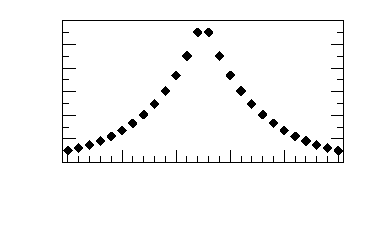
\includegraphics{position_weights}%
\end{picture}%
\begingroup
\setlength{\unitlength}{0.0200bp}%
\begin{picture}(9000,5400)(0,0)%
\put(1250,1500){\makebox(0,0)[r]{\strut{} 0}}%
\put(1250,2067){\makebox(0,0)[r]{\strut{} 2}}%
\put(1250,2633){\makebox(0,0)[r]{\strut{} 4}}%
\put(1250,3200){\makebox(0,0)[r]{\strut{} 6}}%
\put(1250,3767){\makebox(0,0)[r]{\strut{} 8}}%
\put(1250,4333){\makebox(0,0)[r]{\strut{} 10}}%
\put(1250,4900){\makebox(0,0)[r]{\strut{} 12}}%
\put(1630,1000){\makebox(0,0){\strut{} 0}}%
\put(2928,1000){\makebox(0,0){\strut{} 5}}%
\put(4226,1000){\makebox(0,0){\strut{} 10}}%
\put(5524,1000){\makebox(0,0){\strut{} 15}}%
\put(6822,1000){\makebox(0,0){\strut{} 20}}%
\put(8120,1000){\makebox(0,0){\strut{} 25}}%
\put(4875,250){\makebox(0,0){\strut{}$b_{s,k}$}}%
\end{picture}%
\endgroup
\endinput

}}}
\end{picture}
%%
}
\vspace*{-1ex}
\caption{Ranges of values for both $\delta$ and $\omega$ on a typical 
  Affymetrix chip where probes of length~$\ell = 25$ are synthesized in $\mu =
  74$ masking steps. Left: approximate values of the distance-dependent
  weighting function $\delta(s,s',k)$ for a spot~$s$ (shown in the center) and
  close neighbors $s'$, assuming that $s'$ is unmasked at step $k$. Right:
  position-dependent weights $\omega(s,k)$ at each value of $b_{s,k}$,
  assuming that spot $s$ is masked at step $k$.}
\label{fig:conflictindex}
\end{figure}

We note the following relation between conflict indices and border
lengths. Define $\delta(s,s',k):=1$ if $s'$ is a direct neighbor of $s$ and is
unmasked in step $k$, and $:=0$ otherwise; define $\omega(s,k):=1$ if
$s$ is masked in step $k$, and $:=0$ otherwise. Then $\sum_s\, \mathcal{C}(s)
= 2 \sum_{k=1}^\mu\, \mathcal{B}_k$, as each border conflict is counted twice,
once for $s'$ and once $s$. Therefore border length and total conflict are
equivalent for a particular choice of $\delta$ and $\omega$. For our
choice~(\ref{eq:dist_weight}) and~(\ref{eq:pos_mult}), they are not
equivalent, but still correlated: a good layout has both low border lengths and
low conflict indices.


% ==============================================================================
\section{Placement and Partitioning Algorithms}
% ==============================================================================
\label{sec:previous_work}

We now review existing algorithms for microarray layout design. We note that
the placement can be handled by (recursively) partitioning the chip into smaller
regions before applying a placement algorithm. Post-placement optimizations such
as the Chessboard \cite{KAHNG02} are not covered.

\ignore{The first to formally address the border length problem were
\cite{FELDMAN93}. They showed how an optimal placement can be constructed based
on a two-dimensional Gray code. However, their work is restricted to
\emph{uniform arrays} (arrays containing all possible probes of a given length)
and synchronous embeddings.}

\paragraph{Placement Algorithms.}
The border length problem on large oligonucleotide arrays of arbitrary probes
was first formally addressed in~\cite{HANNENHALLI02}. The article reports that
the first Affymetrix chips were designed using a heuristics for the traveling
salesman problem (TSP). The idea consists of building a weighted graph with
nodes representing probes, and edges containing the Hamming distance between
the probe sequences. A TSP tour is approximated, resulting in consecutive
probes in the tour being likely similar. The TSP tour is then
\emph{threaded} on the array in a row-by-row fashion. A different threading of
the TSP tour on the chip, called \emph{1-threading}, is suggested to achieve
up to 20\% reduction in border length~\cite{HANNENHALLI02}.

A different strategy called \emph{Epitaxial} placement
\cite{KAHNG02} places a random probe in the center of the array and continues
to insert probes in spots adjacent to already filled spots. Priority is given
to spots with the largest numbers of filled neighbors. At each iteraction, it
examines all non-filled spots~$s_i$ and finds a non-assigned probe $p_j$ with
minimum sum of Hamming distances $H_{ij}$ to the neighboring probes, employing
a greedy heuristic to select the next spot.  A further 10\% reduction in
border conflict over TSP\,+\,1-threading is claimed.

\ignore{
The major problem with the epitaxial and the TSP-based algorithm is that they
have at least quadratic time complexity and thus are not scalable for the
latest million-probe microarrays. According to their experiments, the TSP
approach needed around 32 minutes to produce the layout of a 200\,x\,200 chip,
whereas the epitaxial algorithm needed 74 minutes on average. For a 500\,x\,500
chip, the TSP took over 30 hours to complete, whereas the epitaxial algorithm
did not complete ``due to prohibitively large running time or memory
requirements'' \cite{KAHNG02}.
}

\ignore{
This observation has led to the development of two new algorithms by
\cite{KAHNG03A}. The first one, called sliding-window matching (SWM), is not
exactly a placement algorithm as it iteratively improves an initial placement
that can be constructed by, for instance, TSP and 1-threading. Improvements
are achieved by selecting an independent set of spots inside the window and
optimally replacing their probes using a minimum-weight perfect matching
algorithm. The term independent refers to probes that can be replaced without
affecting the border length of the other selected probes.
}

Both the Epitaxial algorithm and the TSP approach do not scale well to large
chips. For this reason, \cite{KAHNG03A} proposes a simpler variant of the
Epitaxial algorithm, called \emph{Row-epitaxial}, with two main differences:
spots are filled in a pre-defined order, namely from top to bottom, left to
right, and only probes of a limited list of candidates are considered when
filling each spot. Experiments show that Row-epitaxial is the best
large-scale placement algorithm, achieving up to 9\% reduction in border
length over the TSP\,+\,1-threading.

\paragraph{Partitioning Algorithms.}
The placement problem can be partitioned by dividing the set of probes into
smaller sub-sets, and assigning these sub-sets to sub-regions of the chip.
Each sub-region can then be treated as an independent chip or recursively
partitioned. These smaller sub-problems, when solved, immediately constitute a
final solution. In this way, algorithms with non-linear time or space
complexities can be used to compute the layout of larger chips that otherwise
would not be feasible.

The first known partitioning algorithm is called Centroid-based
Quadrisection~\cite{KAHNG03B}. It starts by randomly selecting a probe
$c_1 \in \mathcal{P}$. Then, it selects another probe $c_2$ maximizing
$h(c_1,c_2)$, the Hamming distance between their embeddings. Similarly, it
selects $c_3$ and $c_4$ maximizing the sum of Hamming distance between these
four probes, which are called centroids. All other probes $p_i \in \mathcal{P}$
are then compared to the centroids and assigned to the sub-set $\mathcal{P}_j$
associated with $c_j$ with minimum $h(p_i,c_j)$. The chip is divided into four
quadrants, each being assigned to a sub-set $\mathcal{P}_j$ .  The procedure
is repeated recursively on each quadrant until a given recursion depth is
reached. In the end, the Row-epitaxial algorithm is used to produce the
placement of the probes in each final sub-region.

We recently developed a novel partitioning approach that, for the first
time, combines the partitioning of the chip with the embedding of the
probes~\cite{CARVALHO06}. Our algorithm, called Pivot Partitioning, achieves
up to 6\% reduction in conflicts when compared to the best known algorithms.

\ignore{
Their results show that the running time of the row-epitaxial algorithm
drops significantly with increasing recursion depth. The time required to place
the probes of a 500\,x\,500 chip, for instance, dropped by 69\% with $L = 3$
when compared with the time required by the row-epitaxial without any
partitioning.
It is not clear from their experiments, however, how the choice of $L$ impaired
the performance of the row-epitaxial algorithm in terms of solution quality
since they have restricted their experiments to $L \leq 3$. Moreover, there is
no clear trend toward reduction or increase in border length as $L$ varies
from~0 to~3.
}

% ==============================================================================
\section{Quadratic Assignment Problem}
% ==============================================================================
\label{sec:qap}

We now explore a different approach to the design of microarrays based on the
quadratic assignment problem (QAP), a classical combinatorial optimization
that can be stated as follows. Given $n \times n$ real-valued matrices $F =
(f_{ij})\geq 0$ and $D = (d_{ij})\geq 0$, find a permutation $\pi$ of $\{1, 2,
\ldots n\}$ such that
\begin{equation}\label{eq:qap_def}
  \sum_{i=1}^{n} \sum_{j=1}^{n}\,  f_{ij} \cdot d_{\pi(i)\pi(j)} \to \min.
\end{equation}

The attribute \emph{quadratic} stems from the fact that the target function
can be written with $n^2$ binary indicator variables $x_{ik}\in\{0,1\}$, where
$x_{ik}:=1$ if and only if $k=\pi(i)$. The objective~(\ref{eq:qap_def}) then
becomes
$
  \sum_{i=1}^{n} \sum_{j=1}^{n}\,  f_{ij} \cdot 
  \sum_{k=1}^{n} \sum_{l=1}^{n}\,  d_{kl} \cdot x_{ik}\cdot x_{jl}
  \to \min,
$
such that $\sum_{k}\, x_{ik}=1$ for all $i$, $\sum_{i}\, x_{ik}=1$ for all $k$
and $x_{ik}\in\{0,1\}$ for all $(i,k)$. The objective function is a quadratic
form in $x$.

The QAP has been used to model a variety of real-life problems. One of its
major applications is to model the facility location problem where $n$
facilities must be assigned to $n$ locations. In this scenario, $F$ is called
the flow matrix as $f_{ij}$ represents the flow of materials from facility $i$
to facility $j$. One unit of flow is assumed to have an associated cost
proportional to the distance between the facilities. Matrix $D$ is called the
distance matrix as $d_{kl}$ gives the distance between locations $k$ and $l$.
The optimal permutation $\pi$ defines a one-to-one assignment of facilities to
locations with minimum cost.

\paragraph{QAP Formulation of Probe Placement.}
The probe placement problem can be seen as an instance of the QAP, where we
want to find a one-to-one correspondence between spots and probes.
%%
\ignore{
To
formulate it, we use the facility location example by viewing the probes as
locations and the spots as facilities, i.e., the spots are assigned to the
probes. In this case the flow matrix $F$ contains the ``closeness'' values
between spots, and the distance matrix $D$ contains the (weighted) Hamming
distances between probe embeddings.  We first give the general formulation for
conflict index; the case of border length minimization is obtained by using
the particular weight functions given at the end of
Section~\ref{sec:model}.
}
%%
In a realistic setting, we may have more spots available than probes
to place. Below we show that this does not cause problems as we can add enough
``empty'' probes and define their weight functions appropriately.

Perhaps more severely, we assume that all probes have a single pre-defined
embedding in order to force a one-to-one relationship.  A more elaborate
formulation would consider all possible embeddings of a probe, but then it
becomes necessary to ensure that only one embedding of a probe is assigned to
a spot. This still leads to a quadratic integer programming problem, albeit
with slightly different side conditions.

Our goal is to design a microarray minimizing the sum of conflict indices over
all spots $i$, i.e., $\sum_{i} \mathcal{C}(i) \to \min$.

The ``flow'' $f_{ij}$ between spots $i$ and $j$ depends on their Euclidean distance
$d(i,j)$ on the array; in accordance with the conflict index model, we set
\begin{equation}
  f_{ij} := \left\{ \begin{array}{ll}
      (d(i,j))^{-2} & \mbox{if spot $j$ is ``near'' spot $i$}, \\
      0 & \mbox{otherwise}. \\
    \end{array} \right.
\end{equation}
%%
where ``near'' means that spot~$j$ is at most three cells away from~$i$. Note
that most of the flow values on large arrays are zero. For Border Length
Minimization, the case is even simpler: We set $f_{ij}:=1$ if spots $i$ and
$j$ are direct neighbors, and $f_{ij}:=0$ otherwise.

The ``distance'' $d_{kl}$ between probes $k$ and $l$ depends on the (weighted) Hamming
distance of their embeddings. To account for possible ``empty'' probes to fill
up surplus spots, we set $d_{kl}:=0$ if $k$ or $l$ or both refer to an empty
probe (i.e., empty probes never contribute to the target function, we do not
mind if nucleotides are erroneously synthesized on spots assigned to empty
probes). For real probes, we set
\[ d_{kl} := \sum_{t=1}^\mu\, d_{klt}, \]
where we now use $t$ as the synthesis step index (the $k$ used in
Section~\ref{sec:model} is now a probe index). The number $d_{klt}$ is the
potential contribution of probe $l$'s embedding to the failure risk of probe
$k$ in the $t$-th synthesis step. According to the conflict index model,
\[ d_{klt}  = \left\{ \begin{array}{ll}
    c \cdot \exp(\theta \cdot \lambda'(k,t)) 
    & \mbox{if $k$ is masked and $l$ unmasked in step $t$,}\\
    0
    & \mbox{otherwise.}
  \end{array} \right.
\]
Because of the change in notation and reference to probes instead of spots, we
repeat that $\lambda'(k,t) = 1 + \min(b'_{k,t},\ell'_{k} - b'_{k,t})$, where
$\ell'_{k}$ is the length of $p_k$ and $b'_{k,t}$ is the number of nucleotides
of $p_k$ synthesized up to and including step $t$.

In the special case of the Border Length Minimization Problem, where
$\theta=0$ and $c=1/2$, we obtain that $d_{kl} + d_{lk} = H_{kl} = H_{lk}$,
where $H_{kl}$ denotes the  Hamming distance between the embeddings of probes
$k$ and $l$.

%% \paragraph{Proof of correctness.}
It now follows that for a given assignment $\pi$, we have
$f_{ij} d_{\pi(i)\pi(j)} = \sum_{t=1}^\mu\, \delta(i,j,t) \cdot \omega(i,t)$
in the notation of Section~\ref{sec:model}. The objective
function~(\ref{eq:qap_def}) then becomes
\begin{eqnarray*}
  & & \sum_i \sum_j\, f_{ij} \cdot d_{\pi(i)\pi(j)} = \sum_i \sum_j\, \left( \sum_{t=1}^\mu\, \delta(i,j,t) \cdot \omega(i,t) \right)\\
  &=& \sum_i \sum_{t=1}^\mu\, \left( \omega(i,t) \cdot \sum_j\, \delta(i,j,t) \right) = \sum_i \mathcal{C}_i,\\
\end{eqnarray*}
and indeed equals the total conflict index with our definitions of $(f_{ij})$
and $(d_{kl})$.
%%
%% \paragraph{Remark.} 
Note that it is technically possible to switch the definitions of $F=(f_{ij})$
and $D=(d_{kl})$, i.e., to assign probes to spots, without modifying the
problem formulation, but this would lead to high distance value for
neighboring spots and many zero distance values for independent spots, a somewhat
counterintuitive model. Also, QAP heuristics tend to find pairs of objects with
large flow values and place them close to each other, initially. Therefore, the
way of modeling $F$ and $D$ may be significant.

\paragraph{QAP Heuristics.}
\ignore{
In the previous sub-section we showed how the microarray placement problem can
be modeled as a quadratic assignment problem. This is interesting because we can
now use existing QAP algorithms to design the layout of microarrays minimizing
either the sum of border lengths or conflict indices. 
}
%%
The QAP is known to be NP-hard and particularly hard to solve in practice.
Instances of size
larger than $n = 20$ are generally considered to be impossible to solve (to
optimality). Fortunately, several heuristics are available.

\ignore{
including
approaches based on tabu search, simulated annealing and genetic algorithms
(see \cite{CELA98}, for a survey).
}

We used a QAP heuristics called GRASP~\cite{LI94} (Greedy Randomized Adaptive
Search Procedure), and an improved version called GRASP with
path-relinking~\cite{OLIVEIRA04} to experimentally validate our formulation.
GRASP is comprised of two phases: a construction phase where a random feasible
solution is built, and a local search phase where a local optimum in the
neighborhood of that solution is sought.

Initially, the elements of the distance and flow matrices are sorted in
increasing and decreasing order, respectively. The first $\beta$ elements
of each are kept (where $0 < \beta < 1$) and their products are computed.
A simultaneous assignment of a pair of facilities to a pair of locations
is selected at random among those with the $\alpha$ smallest costs, where
$0 < \alpha < 1$. A feasible solution is then built by making a series of greedy
assignments.

\ignore{
In the description that follows we use
the terms of the facility location problem: $f_{ij}$ is the flow between
facilities $i$ and $j$, $d_{kl}$ is the distance between locations $k$ and
$l$.

Before the first iteration, GRASP sorts the $(n^2 - n)$ elements of the
distance matrix in increasing order, keeping the first $N:= \lfloor \beta (n^2 -
n) \rfloor$, where $0 < \beta < 1$ is a restriction parameter.
%%
\begin{displaymath}
d_{k_1 l_1} \le d_{k_2 l_2} \le \cdots \le d_{k_N l_N},
\end{displaymath}
%%

It also sorts the $(n^2 - n)$ elements of the flow matrix in decreasing order,
again keeping the first $N$:
%%
\begin{displaymath}
f_{i_1 j_1} \ge f_{i_2 j_2} \ge \cdots \ge f_{i_N j_N}.
\end{displaymath}

Finally, it sorts the costs of assigning initial pairs of facilities to pairs
of locations: The cost of initially assigning facility $i_q$ to location $k_q$
and facility $j_q$ to location $l_q$
for some $q\in\{1,\ldots,N\}$ is $d_{k_q l_q} f_{i_q j_q}$. GRASP sorts
the vector
%%
\begin{displaymath}
(d_{k_1 l_1}  f_{i_1 j_1},\;
d_{k_2 l_2}  f_{i_2 j_2},\; \ldots,\;
d_{k_N, l_N}  f_{i_N j_N}),
\end{displaymath}
%%
keeping the $\lfloor \alpha N \rfloor$ smallest elements, where $0 < \alpha <
1$ is another restriction parameter.

The construction phase of GRASP consists of two stages. In the first stage,
the algorithm makes a simultaneous assignment selected at random among those
with the $\lfloor \alpha \beta (n^2 - n) \rfloor$ smallest costs.

In the second stage of the construction phase, GRASP builds a feasible
solution by making a series of greedy assignments as follows. First, it
computes the costs of all $m$ remaining possible assignments with respect to
assignments already made. Then, it randomly selects one assignment among those
with $\lfloor \alpha m \rfloor$ smallest costs.

In the local search phase, GRASP searches for a local optimum in the
neighborhood of the constructed solution. Different search strategies and
different definitions of the neighborhood can be used. One possible approach is
to check every possible swap of assignments and make those which improve the
current solution until no further improvements can be made.

The best
solutions are kept, but GRASP takes no advantage of the knowledge gained in
previously iterations to build or improve a new solution. This is exactly where
the concept of path-relinking comes into play.
}

The construction and local search phases are repeated for a given number of
times. Each iteration is independent in the sense that a new solution is always built
from scratch. GRASP with path-relinking is an extension of the basic algorithm
that uses an elite set $P$ to store the best solutions found. It incorporates
a third phase that chooses one elite solution at random that is used
to improve the solution produced at the end of the local search phase.

\ignore{
Solutions $p$ and $q$ are combined as follows. For every location
$k = 1, \ldots, n$, the path-relinking algorithm attempts to exchange facility
$p_k$ assigned to location $k$ in  solution $p$ with facility $q_k$ assigned to
location $k$ in the elite solution. In order to keep the solution $p$ feasible,
it exchanges $p_k$ with $p_l$, where $p_l = q_k$. This exchange is
performed only if it results in a better solution. The result of the
path-relinking phase is a solution $r$ that is as good as $p$ and $q$.
For more details on GRASP with path-relinking, we refer to~\cite{OLIVEIRA04}.
}

% ==============================================================================
\section{Results and Discussion}
% ==============================================================================
\label{sec:results}

We present experimental results of using GRASP with path-relinking (GRASP-PR)
for designing the layout of small artificial chips, and compare them with the
layouts produced by Row-epitaxial. We used a C implementation of GRASP-PR provided
by~\cite{OLIVEIRA04} with default parameters (32 iterations, $\alpha=0.1$,
$\beta=0.5$, and elite set with size $|P|=10$) and our own implementation of
Row-epitaxial. The running times and the border length of the resulting layouts are
shown in Table \ref{tab:graspr_reptx}.

\ignore{
The main routine takes
three arguments: matrices $F$ and $D$ and the dimension of the problem~$n$ (in
our case, the number of spots or probes). We generated the matrices using the
formulations presented in Section \ref{sec:qap}.
}

\begin{table}[t]
\caption{Border length of random chips compared with the layouts produced by
Row-epitaxial and GRASP with path-relinking. Reductions in border length are
reported in percentages compared to the initial layout. Chips contain 25-base
long probes uniformly generated and synchronously embedded. Border length and
running times are averages over a set of five chips.\label{tab:graspr_reptx}}
\vspace*{2ex}
\scriptsize{
\begin{tabular}{crrcrrrcrrr}
          &            & Random & & \multicolumn{3}{c}{Row-epitaxial}  & & \multicolumn{3}{c}{GRASP with path-relinking}  \\ \cline{3-3} \cline{5-7} \cline{9-11}
Chip      & Number of  & Border & & Border & Reduction & Time          & & Border & Reduction & Time   \\
dimension & probes     & length & & length & (\%)      & (sec.)        & & length & (\%)      & (sec.) \\
\hline
6\,x\,6   &  36 & 2\,239.20 & & 1\,942.40 & 13.25 & 0.010 & & 1\,882.40 & 15.93 & 2.991   \\
7\,x\,7   &  49 & 3\,115.20 & & 2\,675.60 & 14.11 & 0.020 & & 2\,621.60 & 15.84 & 7.074   \\
8\,x\,8   &  64 & 4\,202.40 & & 3\,514.00 & 16.38 & 0.024 & & 3\,481.20 & 17.16 & 13.568  \\
9\,x\,9   &  81 & 5\,420.00 & & 4\,471.20 & 17.51 & 0.028 & & 4\,460.40 & 17.70 & 28.076  \\
10\,x\,10 & 100 & 6\,740.40 & & 5\,556.20 & 17.57 & 0.034 & & 5\,536.00 & 17.87 & 55.430  \\
11\,x\,11 & 121 & 8\,212.00 & & 6\,726.80 & 18.09 & 0.040 & & 6\,734.80 & 17.99 & 84.659  \\
12\,x\,12 & 144 & 9\,872.00 & & 7\,975.20 & 19.21 & 0.044 & & 8\,038.00 & 18.58 & 148.196 \\
\hline
%% Experiments were conducted on a Sun Fire V1280 server with 900Mhz UltraSparc III+ processors
%% and 96 Gb of RAM under similar load balances.
\end{tabular}}
\end{table}

\begin{table}[t]
\caption{Average conflict indices of random chips compared with the layouts produced by
Row-epitaxial and GRASP with path-relinking. Reductions in conflict indices are
reported in percentages compared to the initial layout. Chips contain 25-base
long probes uniformly generated and synchronously embedded. Conflict indices and
running times are averages over a set of five chips.\label{tab:graspr_reptx_ci}}
\vspace*{2ex}
\scriptsize{
\begin{tabular}{crrcrrrcrrr}
          &            & Random & & \multicolumn{3}{c}{Row-epitaxial}  & & \multicolumn{3}{c}{GRASP with path-relinking}  \\ \cline{3-3} \cline{5-7} \cline{9-11}
Chip      & Number of  & Border & & Border & Reduction & Time          & & Border & Reduction & Time   \\
dimension & probes     & length & & length & (\%)      & (sec.)        & & length & (\%)      & (sec.) \\
\hline
6\,x\,6   &  36 & 2\,239.20 & & 1\,942.40 & 13.25 & 0.010 & & 1\,882.40 & 15.93 & 2.991   \\
7\,x\,7   &  49 & 3\,115.20 & & 2\,675.60 & 14.11 & 0.020 & & 2\,621.60 & 15.84 & 7.074   \\
8\,x\,8   &  64 & 4\,202.40 & & 3\,514.00 & 16.38 & 0.024 & & 3\,481.20 & 17.16 & 13.568  \\
9\,x\,9   &  81 & 5\,420.00 & & 4\,471.20 & 17.51 & 0.028 & & 4\,460.40 & 17.70 & 28.076  \\
10\,x\,10 & 100 & 6\,740.40 & & 5\,556.20 & 17.57 & 0.034 & & 5\,536.00 & 17.87 & 55.430  \\
11\,x\,11 & 121 & 8\,212.00 & & 6\,726.80 & 18.09 & 0.040 & & 6\,734.80 & 17.99 & 84.659  \\
12\,x\,12 & 144 & 9\,872.00 & & 7\,975.20 & 19.21 & 0.044 & & 8\,038.00 & 18.58 & 148.196 \\
\hline
%% Experiments were conducted on a Sun Fire V1280 server with 900Mhz UltraSparc III+ processors
%% and 96 Gb of RAM under similar load balances.
\end{tabular}}
\end{table}

Our results show that GRASP-PR produces layouts with lower border lengths than
Row-epitaxial on the smaller chips. On 6\,x\,6 chips, GRASP-PR
outperforms Row-epitaxial by $2.5$ percentage points on average when compared to
the initial random layout. On 10\,x\,10 chips, however, this difference drops to
$0.6$ percentage point, while Row-epitaxial generates better layouts on 11\,x\,11
or larger chips.
In terms of running time, Row-epitaxial is faster and shows little variation
as the number of probes grows. In contrast, the time required to compute a
layout with GRASP-PR increases at a fast rate.

Because of the large number of probes on industrial microarrays, it is not
feasible to use GRASP-PR (or any other QAP method) to design an
entire microarray chip. However, we showed that it is certainly possible to use
it on small sub-regions of a chip, which opens up the way for two interesting
alternatives. First, such an approach could be used combined with a partitioning
strategy such as the Centroid-based Quadrisection or our new Pivot Partitioning,
to the design the smaller regions that result from the partitioning.

Second, it could be used to improve an existing layout by reloacting probes
inside a defined region. The idea consists of running it iteratively, inside a
sliding-window. Each iteration produces an instance of a QAP whose size equals
the size of the window. The QAP heuristics can be used to check whether
a different arrangement of the probes inside the window can reduce the conflicts.
For this approach to work, however, we also needs to take
into account the conflicts due to the spots around the window. Otherwise, a
new layout with less internal conflicts could result in an increase of conflicts
on the borders of the window.

A simple way of achieving this is to solve a larger QAP instance
consisting of the spots inside the window as well as those around it. The
spots outside the window obviously must remain unchanged, and that can be done
by fixing the corresponding elements of the permutation $\pi$. Then,
there is no need to compute $f_{ij}$ if spots $i$ and $j$ are both outside the
window, nor $d_{kl}$ if probes $k$ and $l$ are assigned to spots outside the
window.

We have identified the probe placement or microarray layout problem with
general distance-dependent and position-dependent weights as a (specially
structured) quadratic assignment problem. QAPs are notoriously hard to solve,
and currently known exact methods start to take prohibitively long already for
slightly more than $20$ objects, i.e., we barely could solve the problem for
$5\times 5$ arrays. However, the literature on QAP heuristics is rich,
as many problems in operations research can be modeled as QAPs. Here we used
one such heuristic to identify the potential of the
probe-placement-QAP-relation.

\ignore{
It is interesting to extrapolate the times shown on Table~\ref{tab:graspr_reptx}
to predict the total time that would be required to design the layout of
commercial microarrays, if we were to combine GRASP-PR with a partitioning
algorithm. If the partitioning produced 6\,x\,6 regions, 37\,636 sub-regions
would be created from the 1164\,x\,1164 Affymetrix Human Genome U133 Plus 2.0
GeneChip\raisebox{.6ex}{\scriptsize \textregistered}, one of the largest
Affymetrix chips. Since each sub-region takes around 3 seconds to compute with
GRASP-PR, the total time required for designing such a chip would be a little
over 31 hours (ignoring the time for the partitioning itself).
%%
If the partitioning produced 12\,x\,12 regions, 9\,409 sub-regions would be
created and, at 2.4 minutes each, the total time would be more than 16 days.
This is probably prohibitive, although it is certainly possible to reduce the
time of each GRASP-PR execution by running it on faster machines or using a
parallel implementation (GRASP is known to be easily parallelized; see
\cite{LI94}).
%%
Figure~\ref{fig:time_extrapolation} shows similar predictions
based on our results with varying chip dimensions and partitioning sizes.
%%
We believe that solution quality is more important than the running time of a
placement algorithm. Even if an algorithm takes a couple of days to complete,
it is time well spent given that commercial microarrays are likely to be
produced in large quantities. This is specially true when we consider the time
required for the whole design process of a microarray chip. Even customer
designed chips, that usually have a limited number of produced units, are likely
to benefit from a few extra hours of computing time.
}

\ignore{
As mentioned earlier, partitioning is a compromise in solution quality in favor
of running time.
However, it is not clear yet how the choice of the maximum
recursion depth in the Centroid-based Quadrisection can undermine the
effectiveness of the placement algorithms. At the moment, we are investigating
alternative partitioning strategies and evaluating their effects on the quality
of the solutions.
}

\ignore{
\begin{figure}
{\footnotesize \centerline{%GNUPLOT: LaTeX picture with Postscript
\begin{picture}(0,0)%
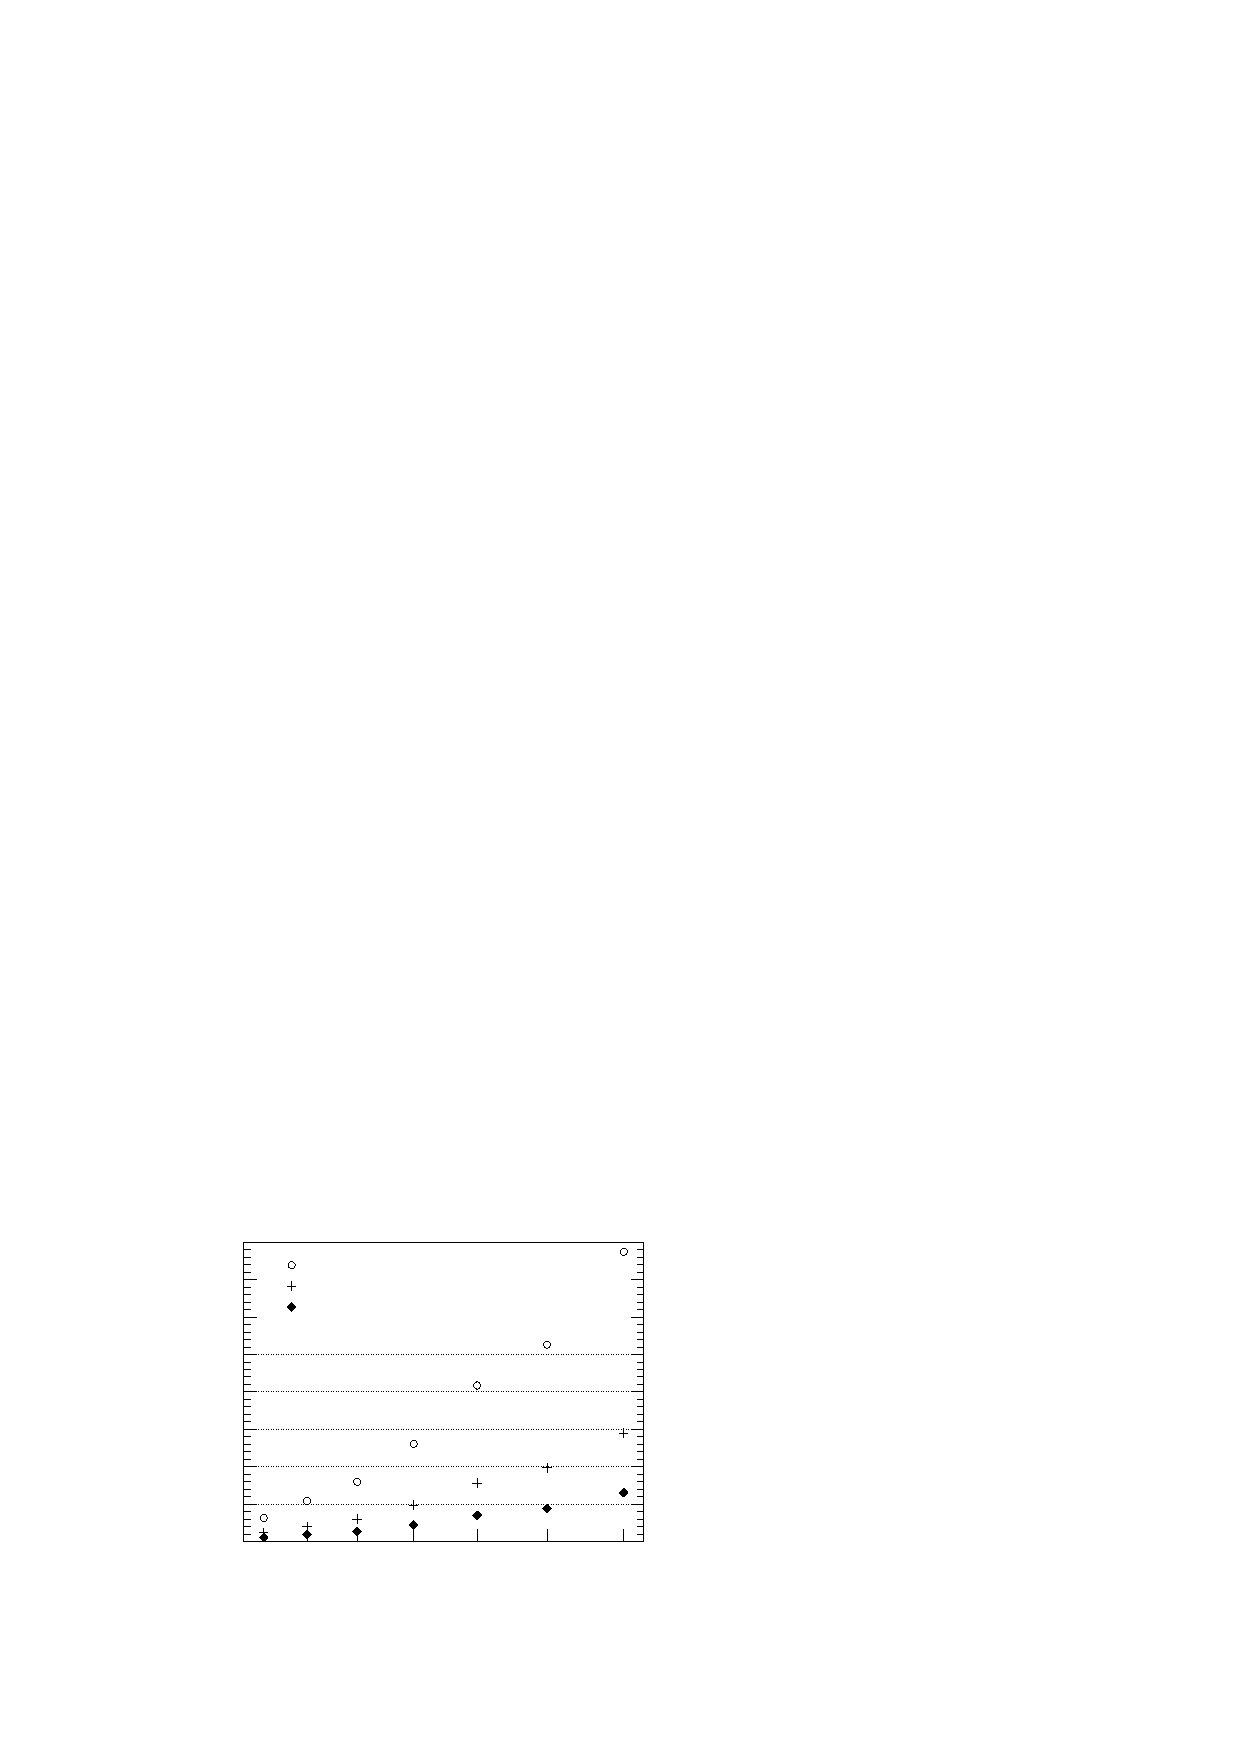
\includegraphics{time_extrapolation}%
\end{picture}%
\begingroup
\setlength{\unitlength}{0.0200bp}%
\begin{picture}(12599,9180)(0,0)%
\put(2000,1500){\makebox(0,0)[r]{\strut{} 0}}%
\put(2000,2397){\makebox(0,0)[r]{\strut{} 50}}%
\put(2000,3295){\makebox(0,0)[r]{\strut{} 100}}%
\put(2000,4192){\makebox(0,0)[r]{\strut{} 150}}%
\put(2000,5090){\makebox(0,0)[r]{\strut{} 200}}%
\put(2000,5987){\makebox(0,0)[r]{\strut{} 250}}%
\put(2000,6885){\makebox(0,0)[r]{\strut{} 300}}%
\put(2000,7782){\makebox(0,0)[r]{\strut{} 350}}%
\put(2000,8680){\makebox(0,0)[r]{\strut{} 400}}%
\put(11370,1000){\makebox(0,0){\strut{}12\,x\,12}}%
\put(9530,1000){\makebox(0,0){\strut{}11\,x\,11}}%
\put(7850,1000){\makebox(0,0){\strut{}10\,x\,10}}%
\put(6330,1000){\makebox(0,0){\strut{}9\,x\,9}}%
\put(4970,1000){\makebox(0,0){\strut{}8\,x\,8}}%
\put(3770,1000){\makebox(0,0){\strut{}7\,x\,7}}%
\put(2730,1000){\makebox(0,0){\strut{}6\,x\,6}}%
\put(500,5090){\rotatebox{90}{\makebox(0,0){\strut{}Hours}}}%
\put(7050,250){\makebox(0,0){\strut{}Maximum dimension of partitions}}%
\put(4300,8130){\makebox(0,0)[l]{\strut{}Human U133 Plus 2.0 (1164\,x\,1164)}}%
\put(4300,7630){\makebox(0,0)[l]{\strut{}Zebra Fish (712\,x\,712)}}%
\put(4300,7130){\makebox(0,0)[l]{\strut{}E.Coli 2.0 (478\,x\,478)}}%
\end{picture}%
\endgroup
\endinput
}}
\caption{Predicted running times required to design selected Affymetrix GeneChip
arrays using GRASP-PR and a partitioning algorithm with varying degrees of
partitioning (based on data shown in Table~\ref{tab:graspr_reptx}). The
dimensions of the chips are shown in parentheses. The time required for the
partitioning itself is ignored.}\label{fig:time_extrapolation}
\end{figure}
}

% ==============================================================================
\begin{thebibliography}{9}
% ==============================================================================

\ignore{
\bibitem{BINDER05} Binder,H. and Preibisch,S. (2005)
Specific and nonspecific hybridization of oligonucleotide probes on microarrays.
{\it Biophysical Journal}, {\bf 89}, 337--352.
}

\bibitem{CARVALHO06}
de Carvalho Jr., S., Rahmann, S.:
Improving the Layout of Oligonucleotide Microarrays: Pivot Partitioning.
Submitted (2006).

\ignore{
\bibitem{CELA98} \c{C}ela,E. (1998) {\it The Quadratic
Assignment Problem: Theory and Algorithms}. Kluwer, Massachessets, USA.
%%
\bibitem{CHASE76} Chase,P.J. (1976) Subsequence numbers and
logarithmic concavity. {\it Discrete Mathematics} {\bf 16}, 123--140.
%%
\bibitem{FELDMAN93} Feldman,W. and Pevzner,P. (1994)
Gray code masks for sequencing by hibridization. {\it Genomics}, {\bf 23},
233--235.
%%
\bibitem{FEO95} Feo,T.A. and Resende,M.G.C. (1995) Greedy
randomized adaptive search procedures. {\it Journal of Global Optimization},
{\bf 6}, 109--133.
}

\bibitem{FODOR91} Fodor,S., Read,J., Pirrung,M.,
Stryer,L., Lu,A. and Solas,D. (1991) Light-directed, spatially addressable
parallel chemical synthesis. {\it Science}, {\bf 251}, 767--73.

\bibitem{HANNENHALLI02} Hannenhalli,S.,
Hubell,E., Lipshutz,R. and Pevzner,P. (2002) Combinatorial algorithms for design
of DNA arrays. {\it Advances in Biochemical Engineering / Biotechnology},
{\bf 77}, 1--19.

\bibitem{KAHNG02} Kahng,A.B., Mandoiu,I.I.,
Pevzner,P.A., Reda,S. and Zelikovsky,A.Z. (2002) Border length minimization in
DNA array design. In {\it Proceedings of the Second Workshop on Algorithms in
Bioinformatics}.

\bibitem{KAHNG03A} Kahng,A.B., Mandoiu,I.,
Pevzner,P., Reda,S. and Zelikovsky,A. (2003a) Engineering a scalable placement
heuristic for DNA probe arrays. In {\it Proceedings of the Seventh Annual
International Conference on Computational Molecular Biology}, 148--156.

\bibitem{KAHNG03B} Kahng, A.B., Mandoiu,I., Reda,S.,
Xu,X. and Zelikovsky,A. (2003b), Evaluation of placement techniques for DNA
probe array layout. In {\it Proceedings of the IEEE/ACM International Conference
on Computer-Aided Design}, 262--269.

\ignore{
\bibitem{KOOPMANS57} Koopmans,T.C. and
Beckmann,M.J. (1957) Assignment problems and the location of economic
activities. {\it Econometrica}, {\bf 25}, 53--76.
}

\bibitem{LI94} Li,Y., Pardalos,P.M. and Resende,M.G.C.
(1994) A greedy randomized adaptive search procedure for the quadratic
assignment problem. In Pardalos,P. and Wolkowicz,H. (eds.), {\it Quadratic
Assignment and Related Problems}, DIMACS Series in Discrete Mathematics and
Theoretical Computer Science, {\bf 16}, 237--261.

\bibitem{OLIVEIRA04} Oliveira,C.A.S., Pardalos,P.M.
and Resende,M.G.C. (2004) GRASP with path-relinking for the quadratic assignment
problem. In Ribeiro,C.C. and Martins,S.L. (eds.), {\it Efficient and
Experimental Algorithms}, Lecture Notes in Computer Science, {\bf 3059},
356--368, Springer-Verlag.

\bibitem{RAHMANN03}
Rahmann,S. (2003) The shortest common supersequence problem in a microarray
production setting. In {\it Proceedings of the 2nd European Conference in
Computational Biology} ({ECCB} 2003), volume 19 Suppl.~2 of
{\it Bioinformatics}, pages ii156--ii161.

\end{thebibliography}

\end{document}



